\documentclass[]{scrartcl}

\usepackage{float}
\usepackage{pgfplots}
\usepackage{xparse}
\usepackage{mathtools}
\usepackage{amsmath}
\usepackage{graphicx} % Required for including pictures
\usepackage{wrapfig} % Allows in-line images
\usepackage{url}
\usepackage{mathpazo} % Use the Palatino font
\usepackage[T1]{fontenc} % Required for accented characters
\linespread{1.05} % Change line spacing here, Palatino benefits from a slight increase by default

\DeclarePairedDelimiter\ceil{\lceil}{\rceil}
\DeclarePairedDelimiter\floor{\lfloor}{\rfloor}
\makeatletter
\newcommand{\mathleft}{\@fleqntrue\@mathmargin0pt}
\newcommand{\mathcenter}{\@fleqnfalse}
\renewcommand\@biblabel[1]{\textbf{#1.}} % Change the square brackets for each bibliography item from '[1]' to '1.'
\renewcommand{\@listI}{\itemsep=0pt} % Reduce the space between items in the itemize and enumerate environments and the bibliography

\renewcommand{\maketitle}{ % Customize the title - do not edit title and author name here, see the TITLE block below
	\begin{center} % Right align
		{\LARGE\@title} % Increase the font size of the title
		
		\vspace{15pt} % Some vertical space between the title and author name
		{\large\@author} % Author name
		\\\@date % Date
		
	\end{center}
}

\usepackage{xcolor}
\usepackage{textcomp}
\definecolor{dkgreen}{rgb}{0,0.6,0}
\definecolor{gray}{rgb}{0.5,0.5,0.5}
\definecolor{mauve}{rgb}{0.58,0,0.82}

\usepackage{listings}

%opening
\title{SPHINCS Interim Report}
\author{Daniel Kirkpatrick\\Vedanth Narayanan}

\begin{document}

\maketitle

\section*{Introduction}
We have been focusing on SPHINCS this whole term. Much of the first couple of weeks was reading documentation adn getting up to speed with the subject and field. There were multiple papers that required time and dedication to fully understand. Understanding the tools and technologies is crucial if we want to be successful. On top of this, we had the added challenge of figuring out how to piece together the technologies, and how SPHINCS uses them.

While we had a lot of catching up to do, we also did get a chance to work on something new. The actual focus is transcribed in this paper. With help from Professor Yavuz, our goal was to come up with a simpler signature scheme that withheld the security that can be incorporated into SPHINCS. The scheme we propose is called Lamport+. On the other hand, we also did some benchmarking to see gauge where SPHINCS stands against RSA and ECDSA.

\section*{Preliminaries}
\vspace{-0.3cm}This section is utilized to briefly talk about existing signature schemes. The sole reason for this is so future references to the specific schemes are not ambiguous. 

\subsection*{Lamport Signature Scheme}
The Lamport Signature Scheme was created by Leslie Lamport in 1989, and it is the simplest signature scheme that exists. It is also the first One-Time signature that was invented. This scheme makes use of a cryptographic hash function that has already been predetermined.\\
To put it simply, the idea behind the scheme can be split into two separate pieces. Signer first generates the secret keys, public keys, hashes messages, and gets a signature that is passed off to the verifier. Now, the verifier's job more or less is to follow similar steps so they end up with a similar result. Thus, it can be argued that the message and signature could only come from the signer and no one else. The detailed version of the scheme is mentioned in the Lamport+ section.

\subsection*{WOTS}
The primary idea behind the scheme is to break the messages into little blocks, that get processed together, and having an input run through a hash function several times. The number of iterations entirely depends on the message that needs to be signed.\\
WOTS was built on top of the Lamport signature scheme, and the expectation is for it to be intuitive in its logic, but it's not the case. The complexity of the scheme is heavily influences by figuring out the number of iterations necessary for a value to go through the hash function.

\subsection*{WOTS+}
WOTS+ is very similar to WOTS, expect for the addition of XORing random elements every time a value is iterated over hash function. In the key generation phase, WOTS+ generates a set of random numbers that will serve for XORing. Just like the keys are split into chunks, so are the random elements. They get incorporated in the following recursive chaining function
\begin{equation}
c_{k}^{i}(x,\textbf{r}) = f_{k}(c_{k}^{i-1}(x,\textbf{r}) \oplus r_{i})
\end{equation}
Th equation is strictly $i > 0$, but in the case of $i = 0$, $c_{0}^{k}(x,\textbf{r}) = x$. The equation is clever in that it makes sure to XOR different values for every iteration. 

\section*{Lamport+ Signature Scheme}
Lamport+ Signature Scheme is the new scheme we are proposing. It not only brings the simplicity of the original Lamport scheme, but also pulls in elements of the WOTS+ scheme. Our hope is that the original scheme's security is withheld, if not enhanced. Please note that the security of the proposed scheme has not been proven, but it can very well be inferred from the previous. Similar to how WOTS+ introduces XORing of randomized elements to WOTS, the same principle is introduced to Lamport. The following is meant to give an idea of how Lamport+ would work as a One Time Signature, before we extrapolate it to hash chains. Take note of the following variables:
\begin{itemize}
	\item $i \in \{0,1\}$, denotes bit pair
	\item $n \in \mathbb{N}$, the security parameter 
	\item $s \xleftarrow{\$} \{0,1\}^m$, seed for the PRNG
	\item PRNG $g : \{0,1\}^m \rightarrow \{0,1\}^n, m < n$
	\item Cryographic hash function $f_k : \{0,1\}^n \rightarrow \{0,1\}^n, k \in \mathcal{K}$
\end{itemize}

\textbf{\underline{Chaining Function}}
\begin{equation}
\begin{split}
c^{i}(x) & = f_{k}(x_{1,n} \oplus g(x_{n+1,n+m})), i > 0 \\
c^0(x) & = x_{1,n}
\end{split}
\end{equation}
The idea for the chaining function, $c : \{0,1\}^{n+m} \rightarrow \{0,1\}^{n}$, is borrowed from WOTS+. Intuitively, the function just splits the seed from the passed in argument, and uses it to XOR a PRN. The subscript, $x_{a,b}$ defines the specific bits used, i.e. $x_a,...,x_b$. $a < b \leq (n+m)$ is assumed to be true.\\ \\
\textbf{\underline{Key Generation}}\\
\textbf{Input:} Security parameter n \\
\textbf{Output:} Secret key $sk$, Public key $pk$
\mathcenter
\begin{equation}
\begin{split}
sk & = ((x_{1}^0, x_{1}^{1}),...,(x_{n}^0, x_{n}^{1}))\\
& = ((c^0_1(x)||s_0,c^0_1(x)||s_1),...(c^0_n(x)||s_0,c^0_n(x)||s_1)), x \in \{0,1\}^{n+m}\\
pk & = ((y_{1}^0, y_{1}^{1}),...,(y_{n}^0, y_{n}^{1})) \\ 
& = ((c^1_1(x_{1}^0)||s_0,c^1_1(x_{1}^1)||s_1),...(c^1_n(x_{n}^0)||s_0,c^1_n(x_{n}^0)||s_1))\\
\end{split}
\end{equation}
\textbf{\underline{Signature Generation}}\\
\textbf{Input:} Secret key $sk$, hashed message $M$ \\
\textbf{Output:} Signature $\sigma$
\mathcenter
\begin{equation}
\begin{split}
\sigma & = (\sigma_1,...,\sigma_n)= (x^{M_1}_1, ..., x^{M_n}_n), M_i \in \{0,1\} \\
\end{split}
\end{equation}
\textbf{\underline{Signature Verification}}\\
\textbf{Input:} Public key $pk$, hashed message $M$, and signature $\sigma$\\
\textbf{Output:} Verification pass or fail
\mathcenter
\begin{equation}
\begin{split}
pk & = (y^i_1,...,y^i_n) \stackrel{?}{=}(c^1_1(\sigma_{1})||\sigma_{n+1,n+m},...,c^1_1(\sigma_{n})||\sigma_{n+1,n+m})
\end{split}
\end{equation}

\subsection*{Lamport+ Hash Chain}
Hash chains aid One-Time signatures to be used multiple times with a single key. This can be applied to the Lamport+ signature scheme. The underlying idea here is that after the public key is generated in the scheme, another set of keys are generated based on the previous public key getting hashed. As you can guess, expect the last public key of the chain, all keys before act as a private key.\\
There are two important things to make note of here. First off, we introduce a new parameter, which we call $l \in \mathbb{N}$, $l > 0$. This parameter helps keep track of how long the chain is, or how many messages can be signed. Secondly, the public keys will hold new PRNG seeds. These seeds will help generate XOR values to help produce the following set of public keys. The concept is better understood once all the steps are explained.\\ \\
\textbf{\underline{Key Generation}}\\
\textbf{Input:} Security parameter n \\
\textbf{Output:} Secret key $sk$, Public key $pk$
\mathcenter
\begin{equation}
\begin{split}
sk_k & = ((x_{1}^{0,k}, x_{1}^{1,k}),...,(x_{j}^{0,k}, x_{j}^{1,k}))\\
& = ((c^k_1(x^{0,k-1}_1)||s_0,c^k_1(x^{1,k-1})||s_1),...,(c^k_j(x^{0,k-1}_j)||s_0,c^k_j(x^{1,k-1}_j)||s_1)), \\
& \hspace{0.7cm} \textrm{where } s\xleftarrow{\$} \{0,1\}^m, 0 \leq k \leq l, 1 \leq j \leq n\\
\end{split}
\end{equation}
Like you could guess, there will no separate public key that will be generated. If the hash chain is properly generated, this is how it should look:
\begin{equation}
\begin{split}
\hspace{-2cm}sk_0 & = ((x_{1}^{0,0}, x_{1}^{1,0}),...,(x_{n}^{0,0}, x_{n}^{1,0})) = ((c^0_1(x)||s_0,c^0_1(x)||s_1),...(c^0_n(x)||s_0,c^0_n(x)||s_1))\\
sk_1 & = ((x_{1}^{0,1}, x_{1}^{1,1}),...,(x_{n}^{0,1}, x_{n}^{1,1})) = ((c^1_1(x_{1}^{0,0})||s_0,c^1_1(x_{1}^{1,0})||s_1),...(c^1_n(x_{n}^{0,0})||s_0,c^1_n(x_{n}^{1,0})||s_1))\\
\vdots\\ 
sk_l & = ((x_{1}^{0,l}, x_{1}^{1,l}),...,(x_{n}^{0,l}, x_{n}^{1,l})) = ((c^1_1(x_{1}^{0,l-1})||s_0,c^1_1(x_{1}^{1,l-1})||s_1),...(c^1_n(x_{n}^{0,l-1})||s_0,c^1_n(x_{n}^{1,l-1})||s_1))
\end{split}
\end{equation}
\textbf{\underline{Signature Generation}}\\
\textbf{Input:} Secret key $sk$, hashed message $M$, Lamport parameter l \\
\textbf{Output:} Signature $\sigma$, Updated Lamport parameter l
\mathcenter
\begin{equation}
\begin{split}
\sigma & = (\sigma_1,...,\sigma_n)= (x^{M_1,l-1}_1, ..., x^{M_n,l-1}_n), M_i \in \{0,1\} \\
l & = l - 1 \\
\end{split}
\end{equation}
\textbf{\underline{Signature Verification}}\\
\textbf{Input:} Public key $pk$, hashed message $M$, and signature $\sigma$\\
\textbf{Output:} Verification pass or fail
\mathcenter
\begin{equation}
\begin{split}
pk & = (y^l_1,...,y^l_n) \stackrel{?}{=}(c^1_1(\sigma_{1})||\sigma_{n+1,n+m},...,c^1_1(\sigma_{n})||\sigma_{n+1,n+m})
\end{split}
\end{equation}

\subsection*{Lamport+ Hash Tree}
The Lamport+ Hash Tree incorporates both the Lamport+ hash chains, and Merkle Hash Trees. The scheme shown here is loosely based on XMSS trees from [6]. The tree allows us sign $\Big(\sum_{i=0}^{2^H-1} l_i\Big)$ messages, with a single global public key. There are some caveats if the tree is going to be used effectively. Signatures are generated from the leftmost chain to the rightmost. To keep track of what the chain the next signature needs to be generated from, we introduce an index variable $i$. Once $i = 2^H-1$, we can determine that signatures for all chains have been used once, and the tree needs to be rehashed using the next set of keys from each of the hash chains. Keep note of the following:
\begin{itemize}
	\item $H$ : Height of tree
	\item $i$ : Index of a node starts from the left and goes to right
	\item $f_k : \{0,1\}^{2n} \rightarrow \{0,1\}^n$
	\item $N : \{0,1\}^{n+m}$, stands for Node
\end{itemize}
\textbf{\underline{Key Generation}}\\
Begin by choosing an $H \geq 1$ variable first. This will allow us to have $2^H$ number of Lamport+ hash chains. The hash chains now need to be created to continue following the algorithm. The following equation shows to construct inner nodes. The leaf nodes will be the hashes of the public key of the hash chains initially. The leaves will change once signatures are generated.\\
\textbf{Input:} $2^H$ hashed public keys of Lamport+ hash chains\\
\textbf{Output:} Lamport+ Hash Tree
\begin{equation}
\begin{split}
N_{i,h} & = f_k((N_{2i,h-1} \oplus g(s_{2i,h-1}))||(N_{2i+1,h-1} \oplus g(s_{2i+1,h-1}))) || s_{i,h} \\
& \textrm{where }0\leq i <2^H, 0 \leq h < H
\end{split}
\end{equation}
\textbf{\underline{Signature Generation}}\\
A signature is first derived the lamport chain, and the tree is reconstructed to take into account the signature. Every time the tree is reconstructed, a new $s \xleftarrow{\$} \{0,1\}^m$ is generated. $A$ is a list of sibling nodes on the path to the tree root. It's important to remember that once a signature is derived, another shouldn't be generated until the first one has been verified. If there is another generated, then the first signature will not properly verify.\\
\textbf{Input:} Hashed message M, lamport chain $l_i$\\
\textbf{Output:} Authentication path A, signature $\sigma_i$, index i
\begin{equation}
\begin{split}
\textrm{if }l_i & > 0, \textrm{ continue, else } i = i+1,\textrm{ start over}\\
\sigma_i & = (x^{M_1,l-1}_1, ..., x^{M_n,l-1}_n)\\
N_{i,h} & = 
\begin{cases}
f_k(\sigma_i||(N_{2i+1,h-1} \oplus g(s_{2i+1,h-1})))||s_{i,h} & ,\textrm{left child} \\
f_k((N_{2i,h-1} \oplus g(s_{2i,h-1}))||\sigma_i)||s_{i,h} & ,\textrm{right child}
\end{cases}
\\A & = (A_0,...,A_{H-1})\\
\end{split}
\end{equation}
\textbf{\underline{Signature Verification}}\\
There are two main steps to look out for here. First, verifying the Lamport+ OTS using the signature that is passed in. Secondly, traversing the hash tree to help check the authenticity for the signature. This algorithm was created with help from [6] and [8].\\
\textbf{Input:} Authentication path A, signature $\sigma$, index i, hashed message M, root node of hash tree $pk$\\
\textbf{Output:} Verification pass or fail\\
\begin{equation}
\begin{split}
sk_l & = (y^l_1,...,y^l_n) \stackrel{?}{=}(c^1_1(\sigma_{1})||\sigma_{n+1,n+m},...,c^1_1(\sigma_{n})||\sigma_{n+1,n+m})\\
P_h & =
\begin{cases}
f_k((P_{h-1} \oplus g(s))||(A_{h-1} \oplus g(s))) \oplus s, & \textrm{if}\floor{\frac{i}{2^h}} \equiv 0 \textrm{ mod }2;\\
f_k((A_{h-1} \oplus g(s))||(P_{h-1} \oplus g(s))) \oplus s, & \textrm{if}\floor{\frac{i}{2^h}} \equiv 1 \textrm{ mod }2;
\end{cases}
,\\ & \textrm{where }0 \leq h < H\\
P_0 & = N_{i,0}\\
pk & \stackrel{?}{=} P_{H-1}
\end{split}
\end{equation}

\subsection*{Security Considerations}
The idea started by looking at the differences between WOTS and WOTS+. They are very similar, so the difference between them is really what makes WOTS+ more secure than the other. The difference all comes down to the fact that WOTS+ performs an Exclusive OR (XOR) operation before a value is hashed. Our job was to take that idea and apply it to Lamport, and ideally the security would be enhanced.

One of the most \textit{elusive} questions in the project was why the authors of WOTS+ XORed random values before hashing values. Even after thoroughly reading the paper multiple times the reason for XORing random values and the security enhancement are not explained. We found out that the paper on XMSS was written only a couple of years before WOTS+, and the author of WOTS+ also coauthored the XMSS paper. It is in XMSS that the idea for XORing random values came from for WOTS+. This operation, once again, is not properly explained in XMSS. The only reference to the bitmasks points to "Collision-resistant hashing: Towards making UOWHFs practical"[7], written by Mihir Bellare and Phillip Rogaway. It was clear that the XOR trick came from them. They have collectively written multiple papers on collision resistant hashing, and key hashing functions. Upon looking through some of the papers, it seemed to first come about in "Keying Hash Functions for Message Authentication" in 1996. This idea was suggested to them by Adi Shamir, one of the cofounders of RSA. Despite the origins of the idea, the thing to take note of is the variety of ways it gets used.

There are two reasons why random values are XORed in the collision-resistant hashing paper. The first reason being able to bring down the key sizes. The more interesting reason is for key scheduling, especially when it comes to compression functions. From our understanding, setting up keys for compression functions can be tedious, so the XOR operations helps with fixing the keys for the "rounds" in a compression function. The security proof was arduous to understand, but the gist is captured here. Essentially, they prove that by using the XOR trick, the compression function is Target-Collision Resistant (TCR). TCR is second preimage resistant, which essentially the Birthday Paradox. 

The following is just a small example. The adversary essentially expects the second collision to be just like the first one, but that is not the case. A new $K$ is introduced in the first collision, and the only way the adversary will get it is by brute forcing it. The adversary needs something to serve as a base, and the adversary does not get that here.
\begin{equation}
\begin{split}
\begin{cases}
XLH_{K,K_1,...,K_j}(M_1,...,M_j) & =  XLH_{K,K_1,...,K_j}(M'_1,...,M'_j)\\
XLH_{K,K_1,...,K_{j-1}}(M_1,...,M_{j-1}) & \neq XLH_{K,K_1,...,K_{j-1}}(M'_1,...,M'_{j-1}) || M'_j\\
\end{cases}
\end{split}
\end{equation}

Like mentioned, WOTS+ makes use of XORing random values. From our understanding, it didn't need to incorporated at all, however it does make the scheme more secure. While there are small overlapping pieces, like hashing values, we don't see a significant necessity for the trick other than to make the scheme a little more unpredictable.

\section*{Testing of SPHINCS, RSA, and ECDSA}
In this section we will be looking at the performance of SPHINCS, RSA, and ECDSA. These three cryptosystems each sign and verify messages in different ways. Below goes into a quick overview on how each system works. Below is a summary of each the cryptosystems we will be looking at. In the next section we will look at how these three cryptosystems match up against each other.

\subsection*{SPHINCS}
SPHINCS makes use of multiple trees to obtain a few time signature (FTS) scheme. This is done using a mixture of Winternitz one time signatures + (WOTS+) and HORS with trees (HORST). The idea of SPHINCS uses a hyper-tree which is borrowed from an idea by Goldreich, which turns a stateful scheme into a stateless scheme. WOTS+ eventually feeds into multiple HORST in the end, which allows for extending signatures to be multi-use instead of single use. SPHINCS has three steps: Key generation, signature generation and signature verification.

\subsection*{RSA}
RSA is used for signing messages by using public-key cryptography. It is an asymmetric cryptosystem that is based on the difficulty of factoring two large prime numbers. With RSA there are four steps we go through: key generation, key distribution, encryption and decryption.

\subsection*{ECDSA}
ECDSA uses elliptic-curve cryptography to obtain the needed parameters. Key generation in ECDSA requires less bits compared to DSA to obtain the same amount of security. The signature size requires the same amount of bit in both ECDSA and DSA to obtain the same amount of security. ECDSA contains three steps: Key generation, signature generation, and signature verification.

\subsection*{Problems with SUPERCOP}
SUPERCOP[12] is a testing suite that is made by Daniel J. Bernstein and Tanja Lange. It contains multiple different types of crypto systems. The problem I was running into with SUPERCOP is that there is no way to run individual testing without having to completely rip the program apart. Dependencies for the most part are in the folders they should be in, but there are a few which I could not find. I had a hard time trying to figure out how to pull out SPHINCS from SUPERCOP because of this problem. Also since SPHINCS could not be pulled from SUPERCOP, I also couldn't figure out how to pull out ED25519.

\subsubsection*{Solution to SUPERCOP problem}
Eventually I did find an implementation that is based on Erlang. The files it uses are taken from SUPERCOP and the author was able to figure out how to make it work using Erlang[13]. Also not being able to use ED25519, I went with using ECDSA from MIRACL as it's the only ECDSA implementation that I have currently available.

\section*{Benchmarks for SPHINCS, RSA, and ECDSA}
Benchmarking is done on Arch Linux (4.4.1-2-ARCH), processor: Intel Quad-Core i7-4710HQ 2.50GHz, 8 gigabytes RAM). The testing for SPHINCS is done using a Erlang implementation which uses code from SUPERCOP. The authors of the SPHINCS paper created SUPERCOP testing suite which benchmarks all different kinds of crypto systems. This implementation is used as trying to compile individual testing from SUPERCOP is very complicated. The testing for RSA and ECDSA is done using MIRACL crypto library, which is an optimized library for performance [11].

The benchmarking is ran using different files sizes, ranging from 10 Kb up to 100 Kb with file sizes being increased in 10 Kb increments. Below you will find two different tests for each cryptosystem, signing and verification.

\begin{table} [H]
	\centering
	\caption{Performance of message signing}
	\begin{tabular}{|c|c|c|c|}
		\hline 
		& SPHINCS & RSA & ECDSA \\ 
		\hline 
		10 Kb & 112.646ms & 0.178332ms & 0.390999ms \\ 
		\hline 
		20 Kb & 113.152ms & 0.140999ms & 0.488332ms \\ 
		\hline 
		30 Kb & 112.445ms & 0.123333ms & 0.670332ms \\ 
		\hline 
		40 Kb & 112.406ms & 0.150666ms & 0.791666ms \\ 
		\hline 
		50 Kb & 112.596ms & 0.156332ms & 1.237333ms \\ 
		\hline 
		60 Kb & 112.875ms & 0.148333ms & 1.320665ms \\ 
		\hline 
		70 Kb & 112.607ms & 0.153999ms & 1.295666ms \\ 
		\hline 
		80 Kb & 112.938ms & 0.162999ms & 1.388666ms \\ 
		\hline 
		90 Kb & 113.241ms & 0.159333ms & 2.458666ms \\ 
		\hline 
		100 Kb & 112.761ms & 0.189666ms & 1.664666ms \\ 
		\hline 
	\end{tabular} 
\end{table}

\begin{table} [H]
	\centering
	\caption{Performance of message verification}
	\begin{tabular}{|c|c|c|c|}
		\hline 
		& SPHINCS & RSA & ECDSA \\ 
		\hline 
		10 Kb & 1.857ms & 0.088666ms & 0.906633ms \\ 
		\hline 
		20 Kb & 1.958ms & 0.140999ms & 1.479999ms \\ 
		\hline 
		30 Kb & 1.935ms & 0.120666ms & 1.398666ms \\ 
		\hline 
		40 Kb & 1.936ms & 0.110333ms & 1.396999ms \\ 
		\hline 
		50 Kb & 2.078ms & 0.137999ms & 1.483999ms \\ 
		\hline 
		60 Kb & 2.053ms & 0.097999ms & 1.659333ms \\ 
		\hline 
		70 Kb & 2.081ms & 0.091666ms & 1.800666ms \\ 
		\hline 
		80 Kb & 2.256ms & 0.118999ms & 1.932999ms \\ 
		\hline 
		90 Kb & 2.323ms & 0.113999ms & 2.053666ms \\ 
		\hline 
		100 Kb & 2.367ms & 0.115666ms & 2.111999ms \\ 
		\hline 
	\end{tabular} 
\end{table}

\begin{center}
	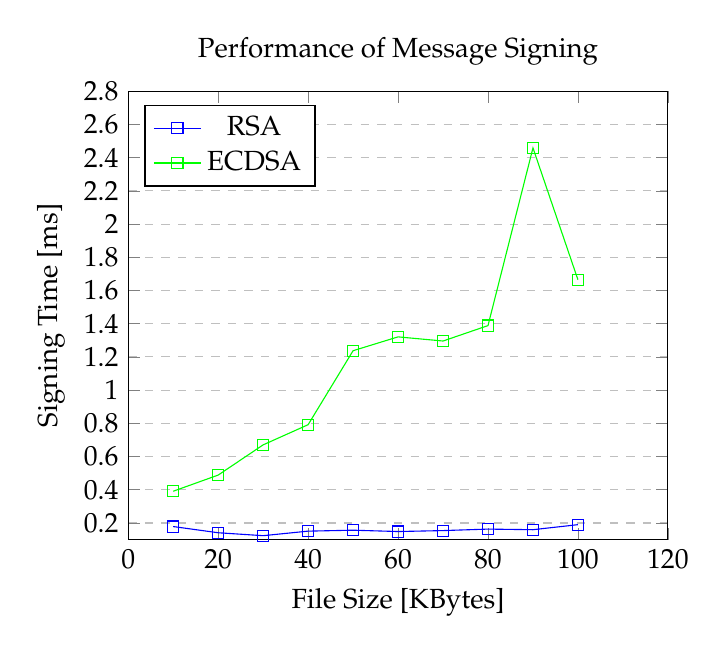
\begin{tikzpicture}
	\begin{axis}[
	title={Performance of Message Signing},
	xlabel={File Size [KBytes]},
	ylabel={Signing Time [ms]},
	xmin=0, xmax=120,
	ymin=0.1, ymax=2.8,
	xtick={0,20,40,60,80,100,120},
	ytick={0, 0.2 ,0.4 ,0.6 ,0.8, 1, 1.2, 1.4, 1.6, 1.8, 2, 2.2, 2.4, 2.6,2.8},
	legend pos=north west,
	ymajorgrids=true,
	grid style=dashed,
	]
	
	\addplot[
	color=blue,
	mark=square,
	]
	coordinates {(10,0.178332)(20,0.140999)(30,0.123333)(40,0.150666)(50,0.156332)(60,0.148333)(70,0.153999)(80,0.162999)(90,0.159333)(100,0.189666)
	};
	
	\addplot[
	color=green,
	mark=square,
	]
	coordinates {(10,0.390999)(20,0.488332)(30,0.670332)(40,0.791666)(50,1.237333)(60,1.320665)(70,1.295666)(80,1.388666)(90,2.458666)(100,1.664666)
	};
	
	\legend{RSA, ECDSA}
	
	\end{axis}
	\end{tikzpicture}
\end{center}

\begin{center}
	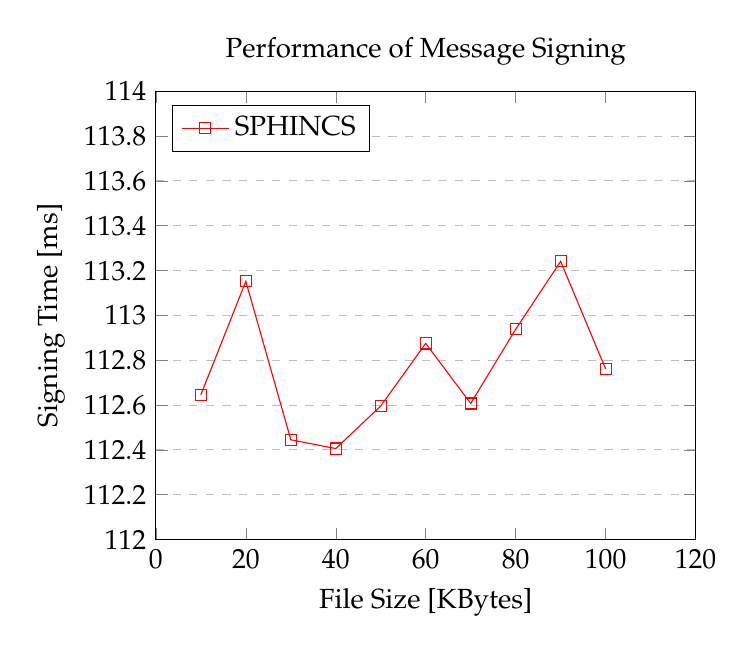
\begin{tikzpicture}
	\begin{axis}[
	title={Performance of Message Signing},
	xlabel={File Size [KBytes]},
	ylabel={Signing Time [ms]},
	xmin=0, xmax=120,
	ymin=112, ymax=114,
	xtick={0,20,40,60,80,100,120},
	ytick={0,112,112.2,112.4,112.6,112.8,113,113.2,113.4,113.6,113.8,114},
	legend pos=north west,
	ymajorgrids=true,
	grid style=dashed,
	]
	
	\addplot[
	color=red,
	mark=square,
	]
	coordinates {(10,112.646)(20,113.152)(30,112.445)(40,112.406)(50,112.596)(60,112.875)(70,112.607)(80,112.938)(90,113.241)(100,112.761)
	};
	
	\legend{SPHINCS}
	
	\end{axis}
	\end{tikzpicture}
\end{center}

\begin{center}
	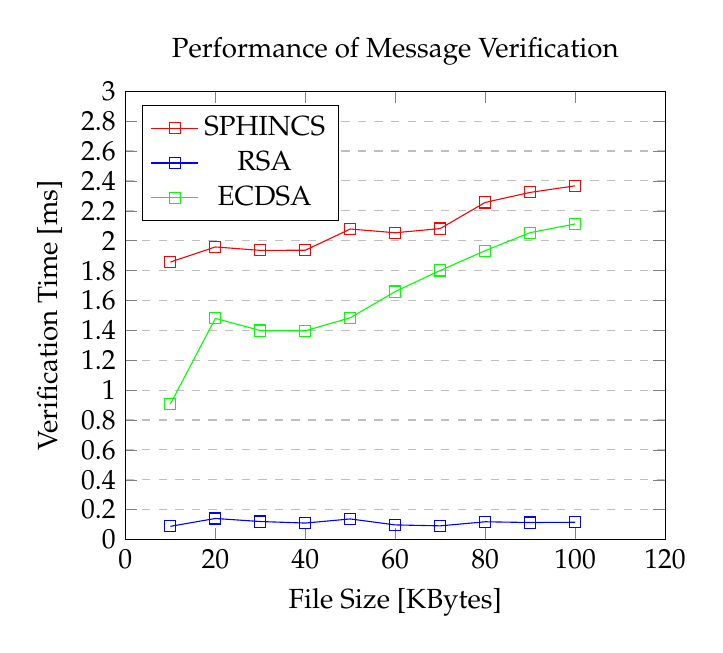
\begin{tikzpicture}
	\begin{axis}[
	title={Performance of Message Verification},
	xlabel={File Size [KBytes]},
	ylabel={Verification Time [ms]},
	xmin=0, xmax=120,
	ymin=0, ymax=3,
	xtick={0,20,40,60,80,100,120},
	ytick={0,0.2,0.4,0.6,0.8,1,1.2,1.4,1.6,1.8,2,2.2,2.4,2.6,2.8,3},
	legend pos=north west,
	ymajorgrids=true,
	grid style=dashed,
	]
	\addplot[
	color=red,
	mark=square,
	]
	coordinates {(10,1.857)(20,1.958)(30,1.935)(40,1.936)(50,2.078)(60,2.053)(70,2.081)(80,2.256)(90,2.323)(100,2.367)
	}; 
	
	
	\addplot[
	color=blue,
	mark=square,
	]
	coordinates {(10,0.088666)(20,0.140999)(30,0.120666)(40,0.110333)(50,0.137999)(60,0.097999)(70,0.091666)(80,0.118999)(90,0.113999)(100,0.115666)
	};
	
	\addplot[
	color=green,
	mark=square,
	]
	coordinates {(10,0.906633)(20,1.479999)(30,1.398666)(40,1.396999)(50,1.483999)(60,1.659333)(70,1.800666)(80,1.932999)(90,2.053666)(100,2.111999)
	};
	
	\legend{SPHINCS, RSA, ECDSA}
	
	\end{axis}
	\end{tikzpicture}
\end{center}


\textbf{NOTE:} Due to SPHINCS performance, signature generation was placed into its own graph.

\section*{Conclusion}
We presented the Lamport+ Signature Scheme along with hash chains and hash trees in this report. The scheme itself is much simpler than both WOTS and WOTS+. The complications arrive when trying to integrate Lamport+ with the Merkle hash trees. Often, hash trees only have one entry for a field, but the nature of a Lamport scheme that's not entirely the case. Based on our algorithm, it is possible to a certain degree, but it's not efficient by any chance. The hash tree algorithm can definitely b more optimized to not only be faster, but costs could be cut doen, and even make a smaller memory footprint. This isn't entirely a promise, but potential future work that would be worth investing time in.

It must stress, as stated in the previous section (Benchmarks), the SPHINCS implementation that was used for this was not optimized at all. The reason for the use of this implementation of SPHINCS was due to ease of use. There are other optimized implementations available, but the complexity to use them is high.

With that being said, as you can see from the graphs above there are trade-offs with using any of these cryptosystems. As file sizes increase the time it takes to sign and verify messages will also increase. 

Based on the implementations used for this benchmark, I would suggest using ECDSA for signatures. ECDSA performs faster than SPHINCS and RSA in terms of signing messages. As you can see though, RSA does verify messages faster than ECDSA, but if you look at the overall performance ECDSA is faster.
\section*{References}
\begin{enumerate}
	\item Merkle, Ralph C. "A certified digital signature." Advances in Cryptology-CRYPTO'89 Proceedings. Springer New York, 1989.
	\item Buchmann, Johannes, et al. "On the security of the Winternitz one-time signature scheme." Progress in Cryptology-AFRICACRYPT 2011. Springer Berlin Heidelberg, 2011. 363-378.
	\item Hulsing, Andreas. "W-OTS+ Shorter signatures for hash-based signature schemes." Progress in Cryptology-AFRICACRYPT 2013. Springer Berlin Heidelberg, 2013. 173-188.
	\item Bernstein, Daniel J., et al. "SPHINCS: practical stateless hash-based signatures." Advances in Cryptology-EUROCRYPT 2015. Springer Berlin Heidelberg, 2015. 368-397.
	\item Buchmann, Johannes, et al. "CMSS - An improved Merkle signature scheme." Progress in Cryptology-INDOCRYPT 2006. Springer Berlin Heidelberg, 2006. 349-363.
	\item Buchmann, Johannes, Erik Dahmen, and Andreas Hulsing. "XMSS-a practical forward secure signature scheme based on minimal security assumptions." Post-Quantum Cryptography. Springer Berlin Heidelberg, 2011. 117-129.
	\item Mihir Bellare and Phillip Rogaway. Collision-resistant hashing: Towards making UOWHFs practical. In Burton Kaliski, editor, Advances in Cryptology - CRYPTO '97, volume 1294 of Lecture Notes in Computer Science, pages 470-484. Springer Berlin / Heidelberg, 1997. 10.1007/BFb0052256.
	\item Erik Dahmen, Katsuyuki Okeya, Tsuyoshi Takagi, and Camille Vuillaume. Digital signatures out of second-preimage resistant hash functions. In Johannes Buchmann and Jintai Ding, editors, Post-Quantum Cryptography, volume 5299 of Lecture Notes in Computer Science, pages 109--123. Springer Berlin / Heidelberg, 2008.
	\item Johannes Buchmann, L. C. Coronado Garcia, Erik Dahmen, Martin Doring, and Elena Klintsevich. CMSS -- an improved Merkle signature scheme. In INDOCRYPT, volume 4329 of Lecture Notes in Computer Science, pages 349--363. Springer, 2006.
	\item https://github.com/joostrijneveld/SPHINCS-py
	\item https://github.com/CertiVox/MIRACL
	\item http://bench.cr.yp.to/supercop.html
	\item https://github.com/ahf/sphincs
\end{enumerate}

\end{document}
